\section{Term-level trends}
\label{sec:analysis}

Motivated by our analysis of updates and change-points, we sought to understand how the language of privacy policies has shifted. While we followed prior research in our use of manually crafted keywords to analyze trends~\cite{degeling2018we},
we additionally developed a system to surface key terms that experts might otherwise overlook. Then we used the key terms surfaced by our tool to guide a more comprehensive analysis into specific concepts.

\subsection{Automated trend surfacing}
\label{sec:automated-trends}

We first built a pipeline to further clean and process the privacy policy texts. We started by replacing certain patterns---URLs, named entities using Spacy~\cite{spacy}, numbers, and emails---in the policies with placeholders. This allowed us to group together phrases that share the same template but include, for example, an organization name. We then extracted terms---n-grams, sentences, named entities, and URLs---for which we obtained the relative document frequency (the percentage of policies they appear in in an interval). Finally, we ranked terms of interest using a variety of scoring functions such as overall gain in relative frequency. 


\begin{table}[]
\centering
\resizebox{\columnwidth}{!}{
\begin{tabular}{rrr}
\toprule
\textbf{2-grams (Gain)}        & \textbf{Entities (Pos Slope 2)} & \textbf{2-grams (Pos Slope 2)} \\ \midrule
service providers (0.27) & gdpr (0.12)             & personal data (0.14)    \\
data protection (0.27)   & eu (0.11)               & data protection (0.13)       \\
personal data (0.24)     & google analytics (0.09) & withdraw consent (0.13)      \\
may include (0.24)       & eea (0.08)              & processing personal (0.13)          \\
may collect (0.22)       & facebook (0.07)         & legitimate interests  (0.12)     \\
\end{tabular}
}
\caption{The top five results from three categories of our automated trend surfacing tool. Scoring functions: ``gain,'' is the difference between the lowest and highest frequency; ``pos slope 2,'' is the maximum slope over any two intervals.}
\label{tbl:automated_results}
\end{table}
\begin{comment}
The trend surfacing tool is intended to surface terms of interest that experts can manually investigate.
It helps in two primary ways. First, it can help us ensure we have not missed any relevant terms during investigations.
Secondly, it can help identify candidate trends that we had not previously considered.
The results from the tool are actionable alone, but they can spark further investigation.\gnote{@RA: are we missing a NOT in the previous sentence?}
\end{comment}

\textbf{Results.} Our trend surfacing tool returned hundreds of phrases which we manually inspected. 
We provide some examples of top-scoring trends that our tool identified in Table \ref{tbl:automated_results}. Under 2-grams measured by gain, we note the growth of terms such as ``may include'' and ``may collect,'' which are terms of ambiguity in privacy policies (previously studied by Reidenberg et al.~\cite{reidenberg2016ambiguity}). This result suggests that privacy policies may be becoming more ambiguous over time, which should be investigated in future work. We noticed growth in terms related to European privacy regulation (GDPR, EU, EEA), along with Google Analytics and Facebook, two commonly used third-party services. We investigate this trend and other trends we observed in more depth in Section~\ref{subsec:trends}. Furthermore, we note growth in terms that likely relate to GDPR.


\subsection{Trends}
\label{subsec:trends}

After examining the results of our automated trend surfacing tool, we chose to investigate trends in three categories: self-regulatory bodies, tracking technologies, and third parties. We investigated tracking technologies because our tool identified several dozen terms of interest related to cookies and web beacons. Similarly, we included third parties as a category because our tool identified terms including Google, Facebook, Instagram, and Twitter. Furthermore, adequate disclosure in each of these categories is crucial to demonstrate the transparency that is a premise of \textit{notice and choice}. Finally, we chose to investigate self-regulatory initiatives because our tool identified several terms containing TrustArc, NAI, and DAA as gaining traction, which may be of interest to regulators.


\begin{figure}
    \centering
    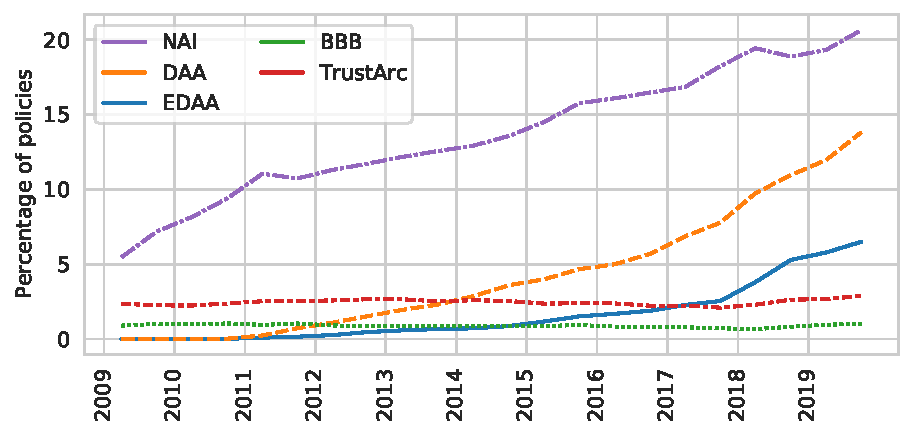
\includegraphics[width=0.9\textwidth]{chapters/privacypolicies/figures/selfreg.pdf}
    \caption{The percentage of policies, after deduplication, referencing self-regulation bodies over time. }
    
%    \Description[Line plot of year vs percentage of policies containing the trend]{The following terms trend roughly linearly upwards, in descending order of final value: NAI, DAA, EDAA. The following terms trend roughly flat: BBB, TrustArc.}
    \label{fig:selfreg}
\end{figure}


\textbf{Self-regulatory initiatives.} 
We began by identifying a set of self-regulatory initiatives. We chose six privacy seal vendors from prior work~\cite{rodrigues2013developing} and three advertising industry trade groups. We then measured how often privacy policies referred to these self-regulatory initiatives, counting a privacy policy as referencing an initiative if it either included the initiative's name or a link to the initiative's website.\footnote{We combined TrustArc and TRUSTe in our analysis, since they are the same entity. Our automated trend detection identified TrustArc as a term with increasing frequency, but when combined with TRUSTe the frequency of references is stable over time.} Figure~\ref{fig:selfreg} plots these references over time, omitting the initiatives that were mentioned in fewer than 1\% of privacy policies.

The graph indicates that self-regulatory online advertising trade groups---the Network Advertising Initiative (NAI), Digital Advertising Alliance (DAA), and European Interactive Digital Advertising Alliance (EDAA)---have seen substantial growth in mentions in privacy policies. The EDAA appears to have more than doubled its presence after the GDPR's introduction, and the NAI has risen around four-fold in 10 years.
By contrast, self-regulatory initiatives that are more commonly associated with first-party websites---
TrustArc and the Better Business Bureau (BBB)---have remained relatively stagnant over time.

\begin{figure}[t]
    \centering
    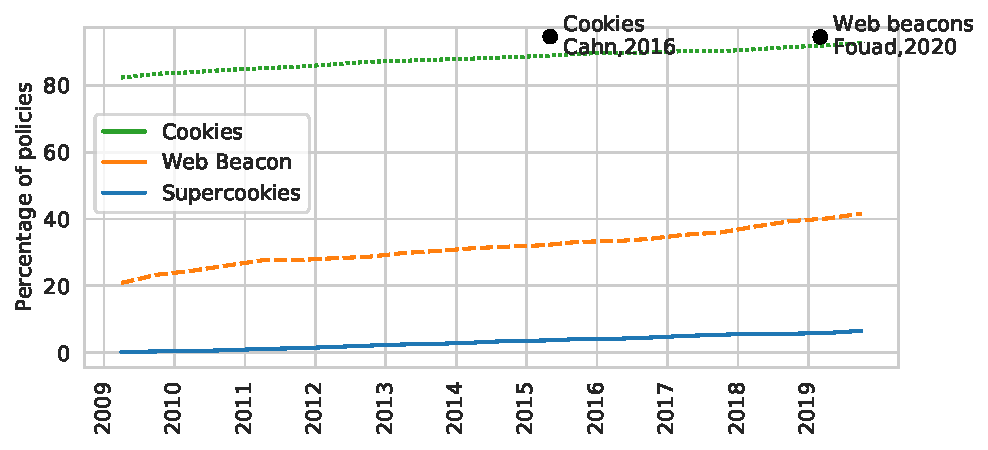
\includegraphics[width=0.9\textwidth]{chapters/privacypolicies/figures/technologies.pdf}
    \caption{The percentage of policies, after deduplication, that reference terms related to stateful tracking technologies. The dot labeled ``Cookies'' is the percentage of websites in the Alexa top 100K with any observed cookies~\cite{cahn2016empirical}. The dot ``Web beacons'' is the percentage of websites in the Alexa top 10K with observed pixels~\cite{Fouad2020missed}.}
%    \Description[Line plot of year vs percentage of policies containing the trend]{The following terms trend slightly upwards, in descending order of final value: cookies, Web Beacon, Supercookies. Other researchers measurements for cookies approximately match the value at that point.}
    \label{fig:trackingtech}
\end{figure}

\begin{figure}[t]
    \centering
    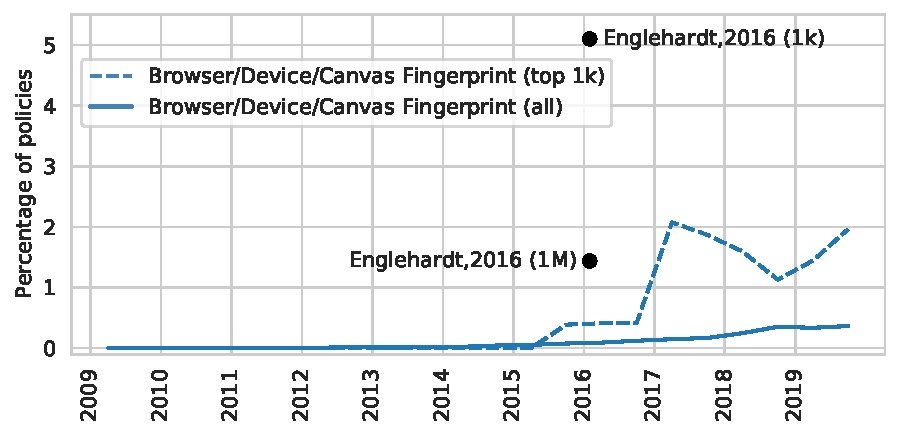
\includegraphics[width=0.9\textwidth]{chapters/privacypolicies/figures/fingerprinting.pdf}
    \caption{The percentage of policies, after deduplication, that reference terms related to fingerprinting. The dot labeled ``1K'' is the percentage of websites in the Alexa top 1K at the time with observed canvas fingerprinting, and ``1M'' is the top 1M~\cite{englehardt2016online}.}
%    \Description[Line plot of year vs percentage of policies containing the trend]{This graph shows Browser/Device/Canvas fingerprinting for all against the top 1k. The top 1k grows faster than all, peaking, then dropping, one year after Englehardt et al., 2016.}
    \label{fig:fingerprinting}
\end{figure}

\textbf{Tracking technologies.} Tracking technologies are pervasive in the modern web~\cite{englehardt2016online}. If privacy policies were fully transparent, we would expect that observations of tracking technologies on the web would match mentions in privacy policies, so we investigated how frequently privacy policies disclose the use of tracking technologies. 

Using our automated trend surfacing tool as a guide, we selected four terms related to tracking technologies, which we split into two categories: stateful tracking technologies and stateless (``fingerprinting'') tracking technologies~\cite{mayer2012}. We constructed regular expressions to match all names listed in the respective Wikipedia entry for the technology~\cite{wikipediaCookie,wikipediaWebBeacon,wikipediaDeviceFingerprint,wikipediaCanvasFingerprint,wikipediaLSO,wikipediaEvercookie}.
The percentage of privacy policies containing the first and second
groups are shown in Figure \ref{fig:trackingtech} and Figure~\ref{fig:fingerprinting}, respectively. Mentions of ``cookie'' are quite close to the observations of the usage of cookies by Englehardt and Narayanan~\cite{englehardt2016online}, and Cahn et al.~\cite{cahn2016empirical}. However, web beacons and fingerprinting appear to be underreported. Fouad et al. measured that 94.6\% of the Alexa top 10K websites had web beacons~\cite{Fouad2020missed}, compared to 25.8\% of policies in 2019 mentioning the related terms. Further, fingerprinting related terms were mentioned far less commonly than Englehardt and Narayanan's measurements of canvas fingerprinting in both the top 1K and top 1M~\cite{englehardt2016online}.

\begin{figure}
    \centering
    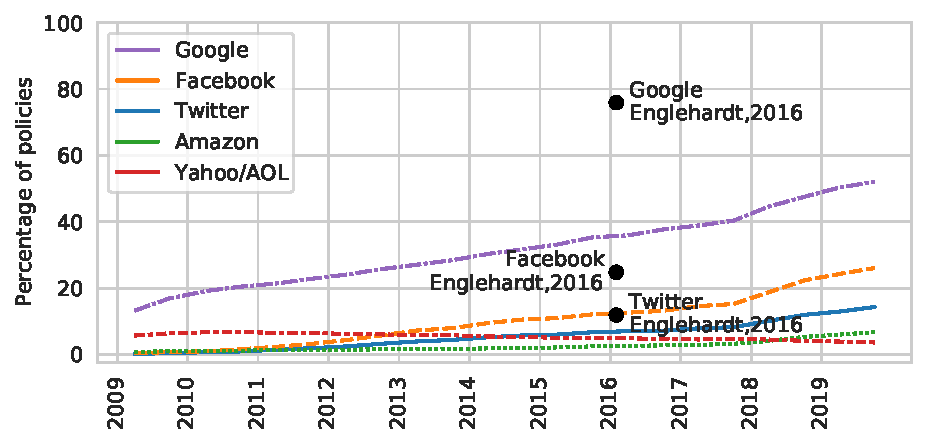
\includegraphics[width=0.9\textwidth]{chapters/privacypolicies/figures/trackers.pdf}
    \caption{The percentage of policies, after deduplication, that reference specific third parties. A match for a common name for the third-party organization, or a match in a link for any domain owned by the third-party organization or their parent organization was considered a reference. Dots indicate measurements of the presence of third parties as a tracker~\cite{englehardt2016online}.}
%    \Description[Line plot of year vs percentage of policies containing the trend]{The following terms trend upwards, in descending order of final value: Google, Facebook, Twitter. The following trends remain flat: Amazon, Yahoo/AOL. Measurements for Twitter from Englehardt et al. are larger but somewhat close to policy mentions. Measurements for Facebook and Google are substantially larger.}
    \label{fig:trackers}
\end{figure}

\textbf{Third parties.} Third-party services are often associated with tracking users on the web~\cite{englehardt2016online}. Continuing our investigation of disclosure and transparency, we chose to examine how often privacy policies disclose the prevalence of third parties.

We compiled a list of 20 popular third parties from other measurements of third parties on the web~\cite{trackerradar, englehardt2016online,lerner2016internet}. We searched for alternative names for each third party and domain names operated by the third party using data from DuckDuckGo's Tracker Radar project~\cite{trackerradar}. We chose the top five most referenced third parties in 2019B, which we show in Figure~\ref{fig:trackers}. We found that these third parties were mentioned in privacy policies far less frequently than they were observed in the web measurements~\cite{trackerradar,englehardt2016online}. 

The gap between observation and disclosure indicates that many privacy policies may not be disclosing all present third parties. 
We note that reporting of third parties is largely increasing. It is unclear if this is due to increased presence or transparency.

\textbf{Validation.} We evaluated our matching criteria for tracking technologies, third parties, and self-regulatory initiatives, to ensure that we were studying the intended trends. Table \ref{tab:selfreg-NDE-labeled} presents results from manually labeling 100 positive examples of each matching category, showing that our matching criteria have high precision.

{
\begin{table}[]
\centering
\resizebox{0.8\columnwidth}{!}{%
\begin{tabular}{@{}lcc@{}}
\toprule
\textbf{Query} & \textbf{Positive} & \textbf{Negative} \\ \midrule
Cookies & 99 & 1\\
Web Beacon & 89 & 11\\
Supercookies & 99 & 1\\
Browser/device/canvas fingerprint& 100 & 0\\
\midrule
Google & 95 & 5\\
Facebook & 86 & 14\\
Twitter & 73 & 27\\
Amazon & 86 & 14\\
Yahoo/AOL & 97 & 3\\
\midrule
TrustArc & 87 & 13\\
BBB & 97 & 3\\
NAI & 95 & 5\\
DAA & 100 & 0 \\
EDAA & 100 & 0\\
\bottomrule
\end{tabular}%
}
\caption{Manual validation of 100 positives for each query. For third parties and tracking technologies, positives indicate the term is used in a context related to tracking. For self-regulatory initiatives, positives indicate a relationship with the initiative.}
\label{tab:selfreg-NDE-labeled}
\end{table}
}

\begin{table}[]
\centering

\resizebox{\columnwidth}{!}{
\begin{tabular}{@{}lrl@{}}
\toprule
\textbf{Privacy policy URL} & \textbf{\# of websites with linking policy} &  \\ \midrule
google.com/privacy\_ads.html & 11,324 &  \\
google.com/intl/en/policies/privacy & 1,690 &  \\
google.com/policies/privacy & 1,421 &  \\
automattic.com/privacy & 948 &  \\
twitter.com/privacy & 931 &  \\
google.com/privacy.html & 873 &  \\
facebook.com/policy.php & 607 &  \\
google.com/privacypolicy.html & 559 &  \\
mailchimp.com/legal/privacy & 528 &  \\
doubleclick.net/us/corporate/privacy & 498 &  \\ \bottomrule
\end{tabular}
}
\caption{Privacy policies that are most linked from the other privacy policies. The right column indicates the distinct number of sites.
}

\label{tab:most-linked-policies}
\end{table}
\textbf{Outbound links.} In addition to disclosing third-party partners, companies may provide links to opt-out pages, industry organizations, or third-party partners that they share data with. Analyzing links found in the privacy policies may reveal trends in third-party data sharing and the effect of regulation on transparency. Here we study links from one privacy policy to another.

We found that 20.3\% of websites link to one or more additional privacy policies. 
This result implies that users wishing to achieve a comprehensive understanding of a website's data practices face an increased burden of reading both the first-party policy and the linked policies.
We show the ten privacy policy URLs with the most incoming links from other policies in Table \ref{tab:most-linked-policies}, which includes six policy URLs from Google. 
  
The privacy links we observe provide an alternate explanation to the disparity we observed in our discussion of tracking technologies
---specific technologies may not be named because they are explained in the third party's privacy policy---instead of the first party's. 



